\documentclass{article}
\usepackage{tikz}
\usetikzlibrary{arrows.meta,positioning,calc,shapes.geometric}
\pagestyle{empty}
\begin{document}
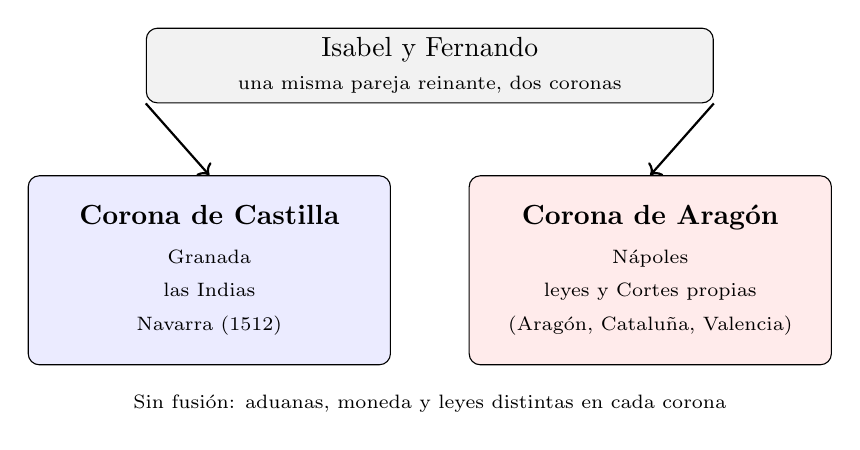
\begin{tikzpicture}
\tikzset{every node/.append style={align=center}}

\node[draw, rounded corners, fill=gray!10, minimum width=7.2cm, minimum height=0.9cm, align=center] (m) at (5.2,3.3) {Isabel y Fernando\\ \scriptsize una misma pareja reinante, dos coronas};
\node[draw, rounded corners, fill=blue!8, minimum width=4.6cm, minimum height=2.4cm, align=center] (c) at (2.4,0.7) {\textbf{Corona de Castilla}\\[2pt] \scriptsize Granada\\ \scriptsize las Indias\\ \scriptsize Navarra (1512)};
\node[draw, rounded corners, fill=red!8, minimum width=4.6cm, minimum height=2.4cm, align=center] (a) at (8.0,0.7) {\textbf{Corona de Aragón}\\[2pt] \scriptsize Nápoles\\ \scriptsize leyes y Cortes propias\\ \scriptsize (Aragón, Cataluña, Valencia)};
\draw[->, thick] (m.south west) -- (c.north);
\draw[->, thick] (m.south east) -- (a.north);
\node[font=\scriptsize, align=center] at (5.2,-1.0) {Sin fusión: aduanas, moneda y leyes distintas en cada corona};

\end{tikzpicture}
\end{document}
